\documentclass[12pt]{article}
\usepackage[utf8]{inputenc}
\usepackage[margin=3cm]{geometry}
\usepackage{float}
\usepackage{graphicx}
\usepackage{physics}
\usepackage{amsmath}
\usepackage{amssymb}
\usepackage[colorlinks]{hyperref}
\usepackage{subcaption}
%\captionsetup{font=footnotesize}
\usepackage{booktabs}
\usepackage{multirow}
\usepackage{newtxtext, newtxmath}
\newcommand{\otoprule}{\midrule[\heavyrulewidth]}
\usepackage[export]{adjustbox}
\usepackage{cite}
\title{Simulation Results for Dyakonov-Shur Instability in the Corbino Geometry}
\author{Jack Farrell}

\begin{document}
	\maketitle
	
	\section{Momentum Relaxation}
	\label{sec:gamma}
	\subsection{Results}
	First, I explored the effect of the momentum-relaxing term. Reference ~\cite{Mendl2019} finds that, for $\eta = 0$, the instability \emph{cannot persist past a certain critical value of $\gamma$}.  
	
		\begin{figure}[ht]
		\centering
		\includegraphics[width=0.8\textwidth]{../../Figures/v0_gamma/v0_gamma.pdf}
		\caption{Dependence of the emitted frequency $f$ on the bias current $v_0$ and the relaxation rate $\gamma$.  The different panes correspond to different values of $\mathcal{R} \equiv L/a$.  For these simulations, $\tilde{\eta} = 0.001$.  The colour white means the instability does not exist.}\label{fig:v0_gamma} 
	\end{figure}

	The first panel of Fig. (\ref{fig:v0_gamma}) makes that property clear --- once the dimensionless $\tilde{\gamma} = \gamma L / v_s$ reaches a value just around $0.75$, we observe no instability for any value of the bias current $v_0$.  But, as we increase $\mathcal{R}=L/a$ through $\mathcal{R} \rightarrow 0$ to $\mathcal{R} = 1.5$, the critical value of $\gamma$ increases.  That means that there is a narrow window of bias currents --- it looks like around $\tilde{v_0} = 0.0 - 0.4$ --- where the instability can persist to higher $\gamma$s than it could in the linear geometry.
	
	Fig. (\ref{fig:v0_gamma}) has a few issues that I am still investigating.  One is the `noise' that appears around the edges of the unstable region, especially in the last two panels.  I am still working on finding a way to more accurately measure the frequency --- my current method is getting confused by some other features in the oscillator.   Another is that an average of five of the $2500$ simulations failed for each plot, and I have not had a chance to re-run them yet, so they show up as white `holes" in the graph.
	
	I also plotted snapshots to illustrate the dynamics of the momentum and density over one period of the oscillator.  Those are given in Fig.(\ref{fig:v0_gamma_snapshots}).
	\begin{figure}[ht]
		\centering
		\includegraphics[width=\textwidth]{../../Figures/v0_gamma/v0_gamma_snapshots.pdf}
		\caption{For $\mathcal{R} = 1.5$ and $\tilde{v_0} = 0.5$, $\tilde{\gamma} = 0.5$, snapshots of $n$ and $J$ over the period of the oscillator.}\label{fig:v0_gamma_snapshots}
	\end{figure}
	
	\subsection{Comparison to Linear Theory}
	The results of Fig.(\ref{fig:v0_gamma}) has some similarities and some differences with the linear theory, and these are summarized in Fig.(\ref{fig:v0_gamma_linear}).  
	
	\begin{figure}[ht]
		\centering
		\includegraphics[width=0.8\textwidth]{../../Figures/v0_gamma_linear.pdf}
		\caption{Results using the linearized equations at the same values as the first two panels of Fig. (\ref{fig:v0_gamma}).}\label{v0_gamma_linear.pdf}
	\end{figure}
	
	The slope of the leftmost edge agrees with the numerics in each plot, but the linear theory fails to predict the disappearance of the instability as $v_0$ is increased to the right, and it also predicts a much less steep decrease in the frequency with $v_0$.  That is to be expected because according to the analytic expression, the dependence on $v_0$ is second order in $v_0$, at least.
	
	\section{Viscosity}
	I also explored the effect of the viscous term.  The simulations here were run at $\tilde{\gamma} = 0.100$, a value estimated by reference ~\cite{Mendl2019} when the channel has length $L \equiv b - a = 1.0\ \mu\text{m}$.
	
	\begin{figure}[H]
		\centering
		\includegraphics[width=0.8\textwidth]{../../Figures/v0_eta/v0_eta.pdf}
		\caption{At $\tilde{\gamma} = 0.100$, the dependence of the emitted frequency on $v_0$ and $eta$.  The colour white means the instability does not exist.}\label{fig:v0_eta}
	\end{figure}
	
	The plot in the first panel of Fig. (\ref{fig:v0_eta}) is close to the one from Fig. 4 of ~\cite{Mendl2019}.  Increasing $\mathcal{R}$ in the other panels, we notice a quick decrease in the frequency.  But the stable region also shifts slightly to the `left' --- this is clear looking at the $\mathcal{R} = 0.005$ panel compared to the $\mathcal{R}=0.001$ panel.  In the third panel, the region translates further to the left, but another effect becomes more clear as well --- the instability disappears for higher $v_0$ if $\eta$ is too large.
	
	These plots still have the same problems as those in Section \ref{sec:gamma}, namely, trouble calculating the frequencies and telling exactly where the instability disappears, and also some failed simulations resulting in missing values.  So I still need to rerun these.
	
	\section{Radius}
	I also wanted to see how the instability depends of $v_0$ and $\mathcal{R}$ exactly --- can you decrease $v_0$ arbitrarily and still observe emitted radiation? That is summarized in Fig. (\ref{fig:v0_ratio}).
	
	\begin{figure}[H]
		\centering
		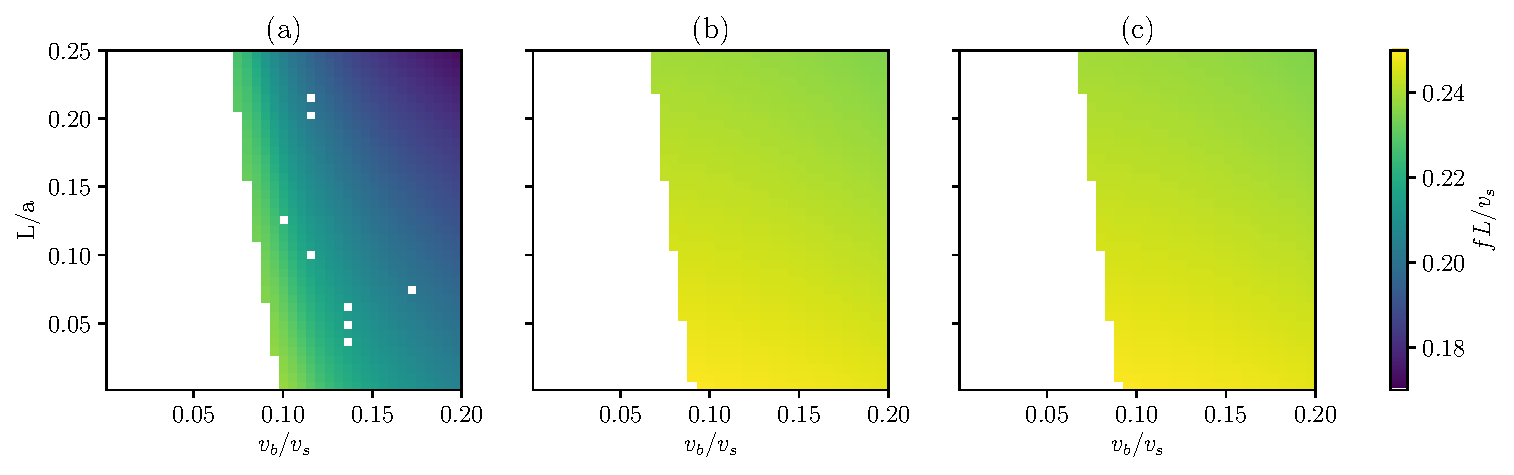
\includegraphics[width=0.5\textwidth]{../../Figures/v0_ratio.pdf}
		\caption{Dependence of the frequency on $\mathcal{R}$ and $v_0$ at $\tilde{\eta}=0.03$ and $\tilde{\gamma} = 0.100$}\label{fig:v0_ratio}
	\end{figure}
	
	
\bibliography{../../References/DSInstability}{}
\bibliographystyle{plain}
\end{document}